\chapter{Introdução} 
\label{sec_Introducao_Dissertacao_orientador}

% Missões espaciais de encontro, acoplamento e atracamento, conhecidas como \gls{rvdb}, desempenham papel central em diversas operações espaciais. Essas missões envolvem a condução de uma espaçonave perseguidora até um veículo alvo em órbita. Operações dessa natureza são empregadas em missões tripuladas, em operações de reabastecimento ou manutenção de satélites e em arquiteturas de serviço em órbita.

Missões espaciais de encontro, acoplamento e atracação, conhecidas como RVD/B, desempenham papel central em operações orbitais modernas. Essas missões permitem o transporte de tripulação, suprimentos e módulos estruturais, além de possibilitarem reabastecimento, manutenção de satélites e montagem de grandes estruturas espaciais, como a \gls{iss} \cite{nasaISS}.

% A execução de uma missão de \gls{rvdb} é normalmente organizada em diferentes etapas, que estabelecem condições para a transição entre as fases da manobra. De forma geral, essas etapas incluem a aproximação inicial, a aproximação de curta distância e a fase final de alinhamento e contato entre as interfaces de acoplamento.

A execução de uma missão de RVD/B é geralmente estruturada em etapas que definem as condições para a transição entre fases da manobra. De forma geral, incluem o lançamento e inserção orbital, o faseamento para reduzir diferenças angulares, a aproximação de longa distância — frequentemente realizada por meio de manobras orbitais como a transferência usando o referencial absoluto (Hohmann) e aproximação de long e  curta distância e de proximidade (final), quando se faz o alinhamento geométrico entre as interfaces de acoplamento, que permite a execução da manobra de docking ou berthing.

O problema de \gls{rvdb} consiste em guiar a espaçonave perseguidora em trajetória relativa até o veículo-alvo, reduzindo progressivamente a distância até que seja possível realizar uma operação segura de acoplamento ou atracação. Essa manobra exige o controle integrado da dinâmica orbital, da atitude e das condições geométricas necessárias para o contato final entre os veículos \cite{curtis2013orbital}.
Durante a aproximação, o perseguidor deve alinhar posição, velocidade relativa e orientação em relação ao alvo, garantindo que as interfaces mecânicas estejam corretamente posicionadas no momento do contato. Em missões não cooperativas, essa operação pode demandar sensores de navegação relativa, algoritmos de controle e, em alguns casos, manipuladores robóticos para realizar a atracação ou estabilização \cite{flores2014review}.

Historicamente, as primeiras demonstrações práticas de operações de rendezvous e docking ocorreram na década de 1960, quando a espaçonave Gemini realizou manobras de aproximação e acoplamento com o veículo-alvo Agena \cite{nasa1stDocking}.
Essas missões estabeleceram os procedimentos básicos para o encontro orbital e demonstraram a viabilidade do controle de trajetória e atitude durante a aproximação \cite{goodman2011rendezvous}.
Posteriormente, o programa Apollo incorporou o docking como parte fundamental da arquitetura de missão, permitindo o acoplamento entre o módulo de comando e o módulo lunar \cite{RVDBapollo,nevins1971}.
Ao longo das décadas seguintes, operações de RVD/B tornaram-se rotineiras em missões tripuladas e robóticas, consolidando-se como capacidade essencial para a exploração espacial. A ISS, por exemplo, depende de operações de docking e berthing para o recebimento de veículos de carga e tripulação \cite{nasaRVDBiss,nasaVisitingVehicles}.

Além das operações clássicas, missões de \gls{rvdb} têm ampliado seu escopo para aplicações modernas, como prestação de serviços em órbita, manutenção de satélites, remoção de detritos espaciais e montagem de grandes estruturas.
Essas aplicações introduzem novos desafios de controle, navegação e interação dinâmica entre veículos espaciais, especialmente em cenários que envolvem alvos não cooperativos ou o uso de manipuladores robóticos \cite{flores2014review,papadopoulos1994}.

A Figura \ref{fig_etapas_rvdb} ilustra as fases típicas de uma missão de \gls{rvdb}.
Inicialmente, ocorre o lançamento do veículo lançador que está carregando a espaçonave perseguidora e a injeta em sua órbita inicial.
Na sequência, a espaçonave perseguidora se mantém em deriva orbital para reduzir a diferença de fase em relação ao alvo.
Em seguida, ocorre a fase de aproximação de curta distância, na qual o controle da posição e da atitude torna-se mais rigoroso.
Por fim, na fase final da operação, o alinhamento geométrico entre as interfaces de acoplamento é realizado, permitindo a execução da manobra de docking ou berthing.

\begin{figure}[H]
\centering
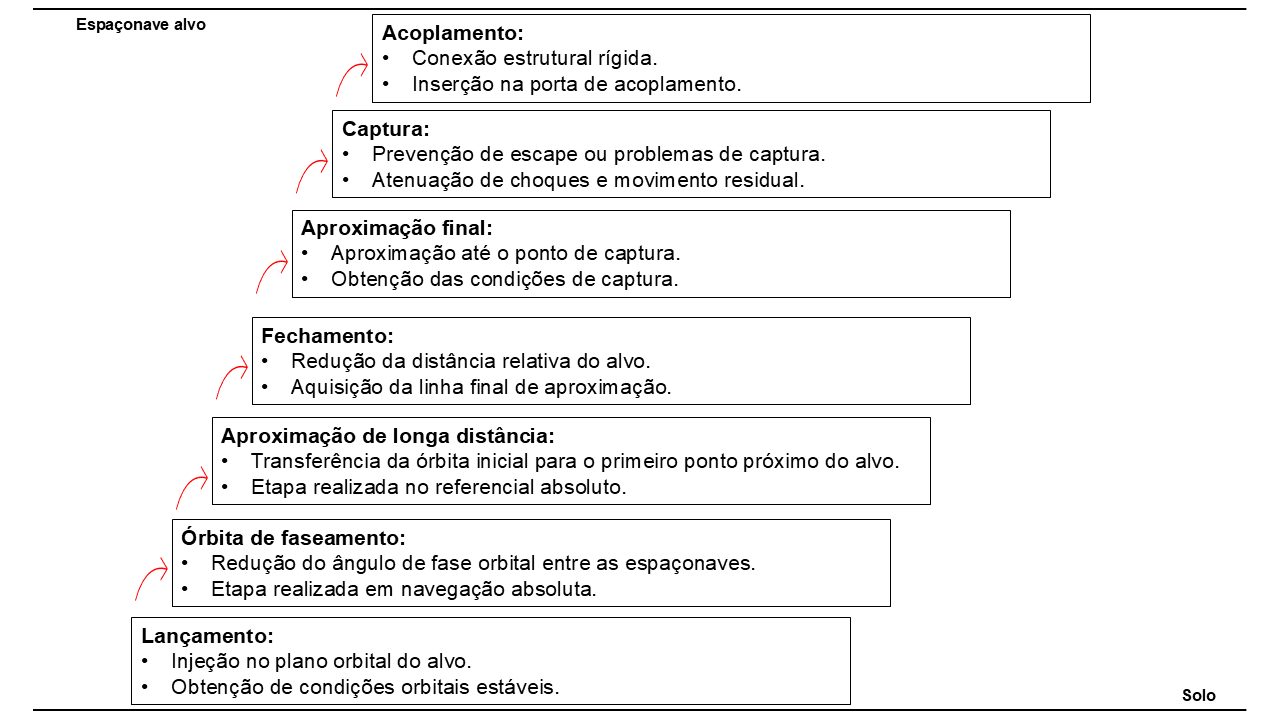
\includegraphics[width=1\linewidth]{4 Formulacao matematica/Imagens/Lançamento quadro explicativo.png}
\caption{Fases de uma missão de \gls{rvdb}, adaptado de \cite{fehse2003}.}
\label{fig_etapas_rvdb}
\end{figure}

\section{Problema do encontro, acoplamento ou atracação}

O problema de \gls{rvdb} consiste em conduzir uma espaçonave perseguidora até um veículo alvo em órbita, reduzindo progressivamente a distância relativa até que seja possível realizar uma operação segura de acoplamento ou atracação.
Essa manobra envolve o controle simultâneo da dinâmica orbital relativa, da atitude da espaçonave e das condições geométricas necessárias para o contato final entre os veículos \cite{curtis2013orbital}.

Durante a aproximação, a espaçonave perseguidora deve executar manobras que permitam alinhar posição, velocidade relativa e orientação em relação ao alvo. 
Essas condições são necessárias para garantir que as interfaces mecânicas envolvidas na operação estejam adequadamente posicionadas no momento do contato.
Em muitas missões, especialmente quando o alvo não coopera ativamente com a manobra, a operação pode exigir o uso de sensores de navegação relativa, algoritmos de controle e, em alguns casos, manipuladores robóticos para realizar a atracação ou estabilização do veículo alvo \cite{flores2014review}.

De forma geral, o problema de \gls{rvdb} pode ser dividido em diferentes fases operacionais, que incluem a aproximação de longa distância a partir de uma órbita próxima, a aproximação de curta distância e a fase final de alinhamento e contato. Cada uma dessas etapas apresenta requisitos específicos de controle, navegação e segurança, tornando necessária a análise integrada da dinâmica orbital e da atitude das espaçonaves envolvidas \cite{fehse2003}.

%%%%%%%%%%%

\subsection{Diferença conceitual entre docking e berthing}

Embora os termos \textit{docking} e \textit{berthing} sejam utilizados de forma conjunta em missões de \gls{rvdb}, eles representam operações distintas \cite{cook2011}.

No \textit{docking}, uma espaçonave executa uma aproximação controlada até a porta de acoplamento do veículo alvo, alinhando os mecanismos de acoplamento até que ocorra o contato entre as interfaces. Após o contato inicial, ocorre a chamada atracação suave (\textit{soft capture}), seguida por processos de amortecimento de cargas e alinhamento estrutural, até que seja estabelecida a conexão estrutural definitiva entre as espaçonaves \cite{cook2011}.

No \textit{berthing}, a aproximação final não é realizada diretamente pela espaçonave perseguidora. Nesse caso, o veículo alvo é capturado por um manipulador robótico e posicionado lentamente em frente à interface de acoplamento da estrutura receptora. Após essa etapa, são realizados processos de alinhamento e fixação estrutural até a conexão final entre os veículos \cite{cook2011}.

Assim, enquanto o \textit{docking} envolve uma aproximação controlada diretamente entre as interfaces de acoplamento das espaçonaves, o \textit{berthing} depende da utilização de um manipulador robótico para capturar e posicionar o veículo antes da fixação final. % ok

\section{Contexto de missões de \gls{rvdb}}

% As missões de \gls{rvdb} permitem que duas espaçonaves realizem acoplamento entre si. Possibilitando transferência de tripulação, reabastecimento, manutenção de satélites e montagem de estruturas espaciais, como a \gls{iss} \cite{nasaISS}.
As operações de \gls{rvdb} envolvem fenômenos dinâmicos que vão além do movimento orbital relativo entre duas espaçonaves. Durante as fases de aproximação próxima e final, a interação entre dinâmica orbital, atitude e movimentação de manipuladores robóticos torna-se determinante para o comportamento da perseguidora. Modelos que consideram apenas o movimento relativo orbital tornam-se insuficientes para descrever essas etapas críticas.

Desde as primeiras missões tripuladas que demonstraram a viabilidade de operações de \gls{rvdb}, o domínio dessas manobras tornou-se uma capacidade essencial para missões espaciais \cite{nasa1stDocking}.
Atualmente, operações de \gls{rvdb} são utilizadas tanto em missões tripuladas quanto em missões robóticas, envolvendo aplicações como prestação de serviços em órbita, captura de satélites inativos \cite{mev_northrop}, remoção de detritos espaciais e montagem de grandes estruturas no espaço.

Essas aplicações ampliam o escopo das operações de proximidade em órbita e introduzem novos desafios de controle, navegação e interação dinâmica entre veículos espaciais.
Em particular, missões que envolvem manipuladores robóticos ou captura de alvos não cooperativos exigem modelos capazes de representar a dinâmica relativa e as interações entre os sistemas envolvidos \cite{papadopoulos1994free,flores2014review}.

%%%%%%%%%%%%%%%%%%%%%%%%%%%%%%%%%%%%%%%%%%%%%%%%%%%%%%
%%%%%%%%%%%%%%%%%%%%%%%%%%%%%%%%%%%%%%%%%%%%%%%%%%%%%%
%%%%%%%%%%%%%%%%%%%%%%%%%%%%%%%%%%%%%%%%%%%%%%%%%%%%%%
\subsection{Evolução das missões de \gls{rvdb}}

As primeiras demonstrações práticas de operações de rendezvous e \textit{docking} ocorreram na década de $1960$, quando a espaçonave \emph{Gemini} realizou manobras de aproximação e acoplamento com o veículo alvo \emph{Agena} \cite{nasa1stDocking}.
Essas missões estabeleceram os procedimentos para operações de encontro orbital e demonstraram a viabilidade do controle de trajetória e atitude durante a aproximação \cite{goodman2011rendezvous}.

Posteriormente, o programa \emph{Apollo} utilizou operações de \textit{docking} como parte fundamental da arquitetura de missão, permitindo o acoplamento entre o módulo de comando e o módulo lunar \cite{RVDBapollo,nevins1971}.
Ao longo das décadas seguintes, operações de \gls{rvdb} tornaram-se rotineiras em missões tripuladas e robóticas, sendo empregada na \gls{iss}, que utiliza operações de \textit{docking} e \textit{berthing} para o recebimento de veículos de carga e tripulação \cite{nasaRVDBiss,nasaVisitingVehicles}.

%%%%%%%%%%%%%%%%%%%%%%%%%%%%%%%%%%%%%%%%%%%%%%%%%%%%%%
%%%%%%%%%%%%%%%%%%%%%%%%%%%%%%%%%%%%%%%%%%%%%%%%%%%%%%
%%%%%%%%%%%%%%%%%%%%%%%%%%%%%%%%%%%%%%%%%%%%%%%%%%%%%%
\subsection{Prestação de serviços em órbita}

Nesse tipo de missão, uma espaçonave de serviço aproxima-se de um satélite alvo para realizar tarefas como inspeção, reabastecimento, atualização de componentes ou extensão da vida útil do veículo \cite{mev_northrop}.

Para que essas missões ocorram, são exigidas capacidades avançadas de navegação relativa e controle durante operações de proximidade, especialmente quando o satélite alvo não foi originalmente projetado para cooperação com operações de captura ou manutenção \cite{arantes2011,flores2014review}.

%%%%%%%%%%%%%%%%%%%%%%%%%%%%%%%%%%%%%%%%%%%%%%%%%%%%%%
%%%%%%%%%%%%%%%%%%%%%%%%%%%%%%%%%%%%%%%%%%%%%%%%%%%%%%
%%%%%%%%%%%%%%%%%%%%%%%%%%%%%%%%%%%%%%%%%%%%%%%%%%%%%%
\subsection{Manutenção}

Operações de manutenção em órbita podem envolver a substituição de componentes, a realização de inspeções ou a correção de falhas em satélites em operação.
Em alguns casos, essas atividades dependem da capacidade de realizar aproximação segura entre veículos e estabelecer contato controlado entre interfaces mecânicas ou manipuladores robóticos \cite{hubbleRVDB,flores2014review}.

%%%%%%%%%%%%%%%%%%%%%%%%%%%%%%%%%%%%%%%%%%%%%%%%%%%%%%
%%%%%%%%%%%%%%%%%%%%%%%%%%%%%%%%%%%%%%%%%%%%%%%%%%%%%%
%%%%%%%%%%%%%%%%%%%%%%%%%%%%%%%%%%%%%%%%%%%%%%%%%%%%%%
\subsection{Remoção de detritos}

A crescente quantidade de detritos espaciais em órbita terrestre tem motivado o desenvolvimento de missões voltadas à captura e remoção de objetos inativos.
Essas missões envolvem a aproximação a alvos não cooperativos, exigindo estratégias robustas de navegação relativa, controle de atitude e mecanismos de captura capazes de lidar com incertezas no estado do objeto alvo \cite{arantes2010,flores2014review}.

%%%%%%%%%%%%%%%%%%%%%%%%%%%%%%%%%%%%%%%%%%%%%%%%%%%%%%
%%%%%%%%%%%%%%%%%%%%%%%%%%%%%%%%%%%%%%%%%%%%%%%%%%%%%%
%%%%%%%%%%%%%%%%%%%%%%%%%%%%%%%%%%%%%%%%%%%%%%%%%%%%%%
\subsection{Montagem espacial}

Operações de montagem em órbita representam outra aplicação importante para missões de \gls{rvdb}.
A construção de estruturas espaciais de grande porte pode exigir o encontro e a integração de múltiplos módulos em órbita, demandando operações sucessivas de aproximação, alinhamento e acoplamento entre veículos ou componentes estruturais \cite{nasaRVDBiss}. % ok

%%%%%%%%%% Motivação
\section{Motivação}

As operações de \gls{rvdb} envolvem fenômenos dinâmicos que não se limitam ao movimento orbital relativo entre duas espaçonaves.
Durante as fases de aproximação de curta distância e fase final, a interação entre dinâmica orbital, atitude e movimentação de manipuladores robóticos passa a desempenhar papel determinante no comportamento da espaçonave perseguidora.
Os modelos que consideram apenas o movimento relativo orbital tornam-se insuficientes para descrever de forma abrangente essas etapas críticas.

Além disso, o crescente interesse em missões de inspeção \cite{dennehy_2016_rcs}, manutenção em órbita \cite{mev_northrop}, remoção de detritos espaciais \cite{jaxa_deb_rendezvous} e montagem de estruturas espaciais, como a \gls{iss}, impõe a necessidade de ferramentas de modelagem que integrem os efeitos dinâmicos associados à presença de um \gls{mr}.
Nesse contexto, torna-se relevante desenvolver uma formulação que una dinâmica orbital relativa e dinâmica acoplada da espaçonave equipada com manipulador, contribuindo para uma representação das operações de \gls{rvdb}.

%%%%%%%%%%%%%%%%%% LIMITAÇÕES
\subsection{Limitações de modelos puramente orbitais para as missões de \gls{rvdb}}

% Modelos baseados exclusivamente na dinâmica orbital relativa são empregados para descrever fases de aproximação de longa distância, assumindo a validade do problema de dois corpos e de um campo gravitacional central, como na Transferência de Hohmann \cite{weberHohmann}.

% Nessa abordagem, a dinâmica é estabelecida apenas pela interação gravitacional, não sendo explicitamente considerados efeitos internos da espaçonave, variações de distribuição de massa ou acoplamentos estruturais.

% Entretanto, nas fases de aproximação de curta distância e na fase final, a movimentação de um \gls{mr} acoplado à espaçonave pode introduzir torques internos e efeitos de acoplamento dinâmico que influenciam diretamente a atitude e a estabilidade do sistema como um todo \cite{nardin2017_simulador}.
% Tais interações tornam-se particularmente críticas quando há necessidade de alinhamento preciso para inserção da ferramenta na interface de acoplamento, uma vez que erros de posicionamento do efetuador final podem ser amplificados pela dinâmica acoplada entre o satélite e o manipulador.

% A desconsideração desses acoplamentos pode conduzir a simplificações que não representam o comportamento dinâmico do sistema durante a interação física com o alvo.
% Assim, evidencia-se a necessidade de incorporar explicitamente a dinâmica acoplada entre a espaçonave e o manipulador na modelagem dessas fases críticas.

Modelos puramente orbitais, baseados na dinâmica relativa em campo gravitacional central, são adequados para fases de longa distância, como a transferência de Hohmann \cite{weberHohmann}.
Entretanto, nas fases próximas, a movimentação de manipuladores robóticos acoplados pode introduzir torques internos e efeitos de acoplamento dinâmico que influenciam diretamente a atitude e a estabilidade do sistema \cite{nardin2017_simulador}. A desconsideração desses efeitos pode levar a simplificações que não representam o comportamento real durante a interação física com o alvo.
Nesse contexto, torna-se essencial integrar a dinâmica orbital relativa com a robótica espacial. A movimentação de manipuladores altera a distribuição de massa e os esforços internos da espaçonave, influenciando sua atitude e seu desempenho dinâmico \cite{yoshida_reactionless_etsvii}.


Essa integração é particularmente relevante em missões de inspeção, manutenção e remoção de detritos, que dependem cada vez mais do uso de manipuladores embarcados.
Exemplos incluem o Canadarm2 na \gls{iss}, utilizado para captura de veículos de carga \cite{canadarm2}, e a missão MEV, responsável pela extensão da vida útil de satélites geoestacionários \cite{mev_northrop}.
O desenvolvimento de modelos integrados contribui para análises de desempenho, avaliação de riscos e planejamento de manobras em cenários operacionais complexos. 

%%%%%%%%%%%%%%%%%% INTEGRAÇÃO
\subsection{Integração entre dinâmica orbital e robótica espacial}

A dinâmica orbital relativa e a robótica espacial são frequentemente tratadas de forma independente na literatura.
Enquanto a primeira descreve o movimento relativo entre espaçonaves em órbita \cite{fehse2003}, a segunda concentra-se na modelagem cinemática e dinâmica de \gls{mr} em microgravidade \cite{yoshida_reactionless_etsvii}.

Entretanto, durante operações de \gls{rvdb}, essas duas áreas interagem diretamente.
A movimentação do \gls{mr} altera a distribuição de massa e os esforços internos da espaçonave, influenciando sua atitude e seu comportamento dinâmico. Essa interação motiva o desenvolvimento de um modelo integrado capaz de representar simultaneamente os fenômenos orbitais e robóticos.


%%%%%%%%%%%%%%%%%% RELEVANCIA
\subsection{Relevância para missões de inspeção, manutenção e remoção de detritos}

Missões de inspeção em órbita, manutenção de satélites, extensão de vida útil e remoção de detritos espaciais dependem cada vez mais do uso de manipuladores robóticos embarcados.
Exemplos incluem o uso do Canadarm2 na \gls{iss} para a captura de veículos de carga \cite{canadarm2}, bem como a missão MEV (Mission Extension Vehicle), responsável pela extensão da vida útil de satélites em órbita geoestacionária \cite{mev_northrop}.

Nessas aplicações, a interação entre movimento orbital relativo e dinâmica do manipulador torna-se parte central do problema, uma vez que a movimentação do \gls{mr} pode influenciar diretamente na atitude da espaçonave durante a operação.

O desenvolvimento de modelos que representem essa integração contribui para a análise preliminar de desempenho, para a avaliação de riscos dinâmicos e para o planejamento de manobras em cenários operacionais complexos. % ok

%%%%%%%%%% Pergunta da pesquisa
\section{Pergunta de pesquisa}
\label{sec_pergunta_pesquisa}

% Diante da complexidade de acoplar e controlar estruturas espaciais em órbita, torna-se necessário investigar ferramentas matemáticas que capturem de maneira fiel as interações dinâmicas do sistema.
% Sendo assim, o presente trabalho é norteado pela seguinte pergunta de pesquisa:
% Como modelar de forma integrada a dinâmica orbital relativa e a dinâmica acoplada de uma \gls{etmr} durante as fases de aproximação de longa distância, aproximação de curta distância e fase final de operações de \gls{rvdb}, de modo fisicamente consistente?

Diante desse desafio, a pergunta de pesquisa que orienta este trabalho é: Como a redistribuição de massa causada pelo movimento de um manipulador robótico influencia a dinâmica relativa, a sincronização de pose e o controle de atitude de uma nave perseguidora durante a fase de aproximação de proximidade em operações de \gls{rvdb}? 
 % ok

%%%%%%%%%% Objetivos (os objetivos não são os objetivos do mestrado mas os objetivos da dissertação)

%%%%%%%%%% Objetivos
\section{Objetivos}
\label{sec_objetivos}

O presente trabalho visa desenvolver e simular um modelo matemático para missões de \gls{rvdb} de forma conjunta a dinâmica orbital relativa e a dinâmica acoplada entre uma espaçonave perseguidora e seu \gls{mr}.
O modelo desenvolvido descreve o movimento relativo nos referenciais ECI e \gls{lvlh}, tratando o perseguidor sob duas abordagens:
(i) como corpo rígido, via Equações de Euler; e
(ii) como sistema multicorpos acoplado, via formulação lagrangiana.
Além da modelagem, o trabalho contempla a implementação de um controle de atitude do tipo \gls{pd} e a simulação computacional em Matlab e Simulink para avaliar os torques de reação induzidos na espaçonave.

A seguir, apresentam-se o objetivo geral e os objetivos específicos que guiam esta dissertação.

%%%%%%%%%%%%%%%%%%%%%%% OBJ GERAL

\subsection{Objetivo geral}
\label{subsec_objetivo_geral}

% Desenvolver e analisar um modelo dinâmico integrado entre a dinâmica orbital relativa e a dinâmica acoplada de uma espaçonave perseguidora equipada com \gls{mr}, aplicado às fases de aproximação de curta distância e final de operações de berthing, incorporando controle de atitude do tipo \gls{pd}, com validação em ambiente de simulação computacional nas plataformas Matlab e Simulink.
Desenvolver e analisar um modelo dinâmico integrado entre a dinâmica orbital relativa e a dinâmica acoplada de uma espaçonave perseguidora equipada com \gls{mr}, aplicado às fases de aproximação de proximidade (final) de operações de berthing, incorporando controle de atitude do tipo \gls{pd} e validado em ambiente de simulação computacional nas plataformas Matlab e Simulink.



%%%%%%%%%%%%%%%%%%%%%%% OBJ ESPECIFICOS

\subsection{Objetivos específicos}
\label{subsec_objetivos_especificos}

% Os objetivos específicos deste trabalho foram organizados de forma a estruturar o desenvolvimento do modelo desde a definição dos requisitos dinâmicos até a análise do comportamento do sistema integrado em simulação, estabelecendo um encadeamento lógico de pesquisa:

% \begin{itemize}
%     \item Identificação das necessidades: Definir os requisitos associados às fases de aproximação de longa e curta distâncias e fase final de uma missão de \gls{rvdb}. Isso inclui caracterizar o comportamento do modelo de corpo rígido (com \gls{mr} travado) e do modelo acoplado (durante o modo operacional), além de identificar variáveis críticas como posição, velocidade relativa e sincronização de atitude com a espaçonave alvo.
    
%     \item Proposta de processo: Estabelecer o modelo matemático capaz de integrar as dinâmicas orbital e acoplada. Esta etapa engloba a formulação do modelo relativo nos referenciais ECI e \gls{lvlh}, a derivação do modelo acoplado via abordagem lagrangiana, e a definição dos parâmetros cinemáticos do \gls{mr} utilizando o método de \gls{dh}.
    
%     \item Aplicação do processo proposto: Implementar as equações desenvolvidas computacionalmente em Matlab e Simulink. O foco desta etapa é integrar os subsistemas orbital, dinâmico e de controle (controlador \gls{pd}) e realizar simulações sob diferentes condições iniciais para observar o comportamento da espaçonave.
    
%     \item Avaliação do processo proposto: Avaliar o comportamento dinâmico do sistema integrado a partir dos resultados simulados. Busca-se analisar a redução da diferença de fase entre as espaçonaves, o perfil de posição e velocidade relativas, o comportamento da atitude do perseguidor frente à operação do \gls{mr} e a eficácia da ferramenta na porta de acoplamento.
% \end{itemize}

Definir requisitos associados às fases de aproximação de longa e curta distância e fase final de uma missão de RVD/B, caracterizando o comportamento do modelo de corpo rígido e do modelo acoplado, além de identificar variáveis críticas como posição, velocidade relativa e sincronização de atitude.

\begin{itemize}
    \item Estabelecer o modelo matemático capaz de integrar as dinâmicas orbital e acoplada, incluindo formulação relativa nos referenciais ECI e LVLH, derivação lagrangiana e definição dos parâmetros cinemáticos do manipulador via método \gls{dh}.
    \item Implementar as equações desenvolvidas em Matlab e Simulink, integrando subsistemas orbital, dinâmico e de controle (PD), e realizar simulações sob diferentes condições iniciais.
    \item Avaliar o comportamento dinâmico do sistema integrado a partir dos resultados simulados, considerando redução da diferença de fase, perfis de posição e velocidade relativas, atitude do perseguidor frente à operação do manipulador e eficácia da ferramenta na interface de acoplamento.
\end{itemize}
 % ok

\subsection{Metodologia}

% A metodologia adotada neste trabalho é de natureza teórico-computacional, fundamentada no desenvolvimento matemático e na validação por meio de simulação numérica.
% Inicialmente, realizou-se uma revisão bibliográfica sobre dinâmica orbital relativa, robótica espacial e operações de \gls{rvdb}, com o objetivo de identificar lacunas na integração entre essas áreas.

% Na sequência, foi desenvolvida uma formulação matemática integrada, contemplando a dinâmica orbital relativa da espaçonave perseguidora em relação à espaçonave alvo e a dinâmica acoplada entre a espaçonave e seu \gls{mr}.
% A modelagem cinemática do manipulador foi conduzida por meio do método de \gls{dh}, enquanto a dinâmica acoplada foi formulada utilizando abordagem lagrangiana baseada na energia cinética do conjunto espaçonave--\gls{mr}.

% O modelo foi implementado computacionalmente em Matlab e Simulink, incluindo a incorporação de lei de controle do tipo \gls{pd} para o movimento orbital, atitude e movimento das juntas do \gls{mr}.
% Para a aproximação de longa distância foram realizadas simulações numéricas para diferentes condições iniciais, que permitiu avaliar o comportamento dinâmico da espaçonave durante esta fase e como iria interferir nas fases seguintes, como a aproximação de curta distância e aproximação final.

% A avaliação dos resultados foi conduzida por meio da análise dos perfis temporais das variáveis orbitais e de atitude, com ênfase na influência do \gls{mr} sobre a dinâmica da espaçonave perseguidora.
% Em resumo, foi realizado o seguinte:

% \begin{itemize}
%     \item Revisão bibliográfica sobre dinâmica orbital relativa, robótica espacial e operações de \gls{rvdb}.
%     \item Desenvolvimento da formulação matemática integrada.
%     \item Modelagem cinemática do \gls{mr} via \gls{dh}.
%     \item Formulação dinâmica acoplada por abordagem lagrangiana.
%     \item Implementação computacional em Matlab e Simulink.
%     \item Implementação de lei de controle \gls{pd}.
%     \item Realização de simulações numéricas sob diferentes condições iniciais.
%     \item Análise qualitativa dos resultados por inspeção dos perfis temporais das variáveis dinâmicas.
% \end{itemize}

A metodologia adotada é de natureza teórico-computacional, fundamentada no desenvolvimento matemático e na validação por meio de simulação numérica. Inicialmente, realizou-se uma revisão da literatura sobre dinâmica orbital relativa, robótica espacial e operações de RVD/B, com o objetivo de identificar lacunas na integração entre essas áreas.
Na sequência, foi desenvolvida uma formulação matemática integrada, contemplando a dinâmica orbital relativa da perseguidora em relação ao alvo e a dinâmica acoplada entre a espaçonave e seu manipulador. 
A modelagem cinemática do manipulador foi conduzida pela convenção de \gls{dh}, enquanto a dinâmica acoplada foi formulada via abordagem lagrangiana baseada na formulação via energia e coordenadas generalizadas. Com essa metodologia derivou-se as equações movimento acopladas energia através do uso da energia cinética do sistema espaçonave tipo manipulador robótico na configuração de corpo não rígido.
O modelo foi simulado computacionalmente em ambiente Matlab e Simulink, incluindo controlador PD para movimento orbital, atitude e juntas do manipulador. Foram realizadas simulações numéricas em diferentes condições iniciais, permitindo avaliar o comportamento dinâmico da perseguidora nas fases de aproximação de longa distância, curta distância e final.
A avaliação dos resultados foi conduzida por meio da análise dos perfis temporais das variáveis orbitais e de atitude, com ênfase na influência do manipulador sobre a dinâmica da perseguidora.
 % ok

\section{Estrutura do documento}

% 1
O Capítulo~\ref{sec_Introducao_Dissertacao}: Introdução ao tema, incluindo contextualização, motivação, pergunta de pesquisa, objetivos e metodologia.

% 2
O Capítulo~\ref{sec_Revisao_bibliografica}: Revisão da literatura, abordando trabalhos relacionados à dinâmica orbital relativa, robótica espacial e modelagem de operações de RVD/B.

% 3
O Capítulo~\ref{sec_Procedimento_simulacao}: Procedimento de simulação, com fluxogramas e organização da implementação computacional.

% 4
O Capítulo~\ref{sec_Formulacao_Matematica}: Formulação matemática, incluindo modelagem orbital, cinemática do manipulador via DH, formulação lagrangiana e controle de atitude.

% 5
O Capítulo~\ref{sec_resultados}: Ambiente de simulação e resultados obtidos para as fases de aproximação de longa distância, curta distância ede proximidade (final)

% 6
O Capítulo~\ref{sec_Discussao}: Discussão dos resultados, destacando comparação com a literatura, contribuições do trabalho, lições aprendidas e limitações.

% 7
O Capítulo~\ref{sec_Conclusao}: Conclusão, incluindo o atingimento dos objetivos, resumo das contribuições, relevância e trabalhos futuros.
